\usetikzlibrary{decorations.text}
\usetikzlibrary{calc}
\usetikzlibrary{fit}
\usetikzlibrary{shapes}
\usetikzlibrary{arrows,positioning}

\begin{figure}[h]
\begin{center}

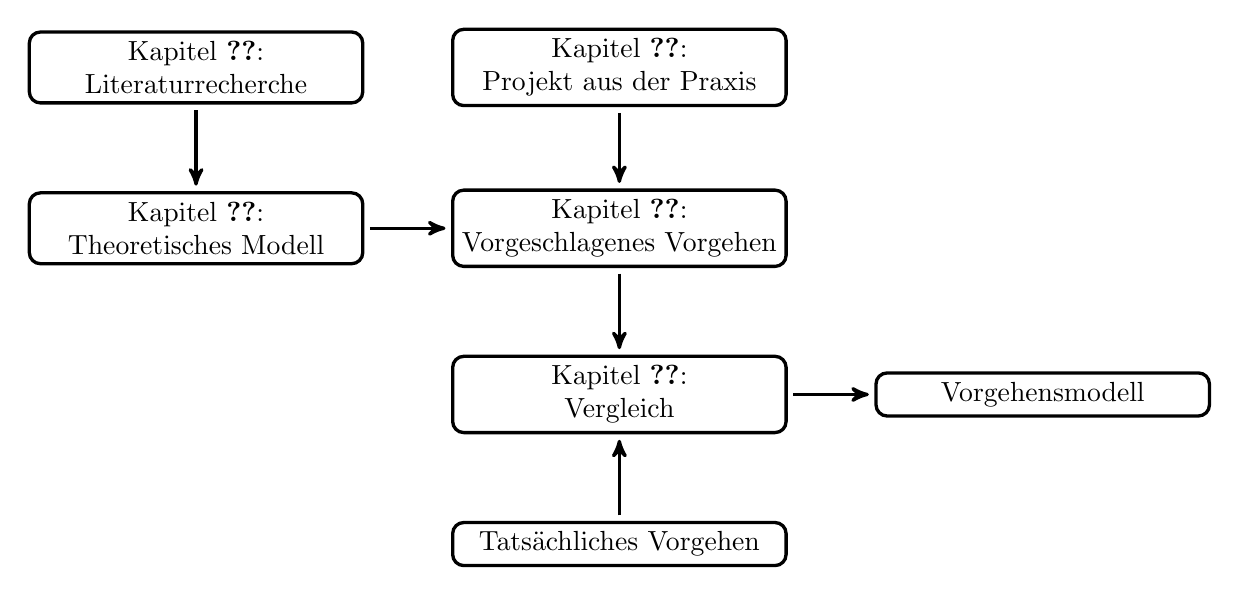
\begin{tikzpicture}[node distance=1.1cm,
auto,
pile/.style={
  very thick,
  ->,
  >=stealth',
  shorten <=2pt,
  shorten >=2pt
},
knoten/.style={
  text width=4cm,
  text centered,
  rectangle,
  very thick,
  draw=black,
  rounded corners,
}]
\node[knoten] (TM) [] {Kapitel~\ref{cha:entwicklung_vorgehensmodell}:\\Theoretisches Modell};
\node[knoten] (L) [above=of TM] {Kapitel~\ref{cha:method}:\\Literaturrecherche};

\draw[pile] (L) -> (TM);
\node[knoten] (VV) [right=of TM] {Kapitel~\ref{cha:result}:\\Vorgeschlagenes Vorgehen};
\node[knoten] (P) [right =of L] {Kapitel~\ref{cha:replyundifms}:\\Projekt aus der Praxis};

\draw[pile] (TM) -> (VV);
\draw[pile] (P) -> (VV);

\node[knoten] (VGL) [below=of VV] {Kapitel~\ref{cha:diskussion}:\\Vergleich};
\node[knoten] (TV) [below=of VGL] {Tatsächliches Vorgehen};

\draw[pile] (VV) -> (VGL);
\draw[pile] (TV) -> (VGL);

\node[knoten] (VM) [right=of VGL] {Vorgehensmodell};

\draw[pile] (VGL) -> (VM);


\end{tikzpicture}

\end{center}
\caption{Gliederung dieser Arbeit; Entwicklung des Vorgehensmodells}
\label{fig:gliederung}
\end{figure}
